\chapter{Manim基本图形}
\section{点}
点是最简单图形，也是其他所有图形的基础。 绘制其他任何图形时，都是用点来定位的。

\begin{lstlisting}[style=demostyle,numbers=none]
Dot([x, y, z])
Dot([x, y, z], color=color)
\end{lstlisting}    

\begin{lstlisting}[style=pythonstyle]
# manim -pql 01Dot_demo.py DotSample    
from manim import *
class DotSample(Scene):
    def construct(self):
        # 绘制 9个点
        for x in range(-1, 2):
            for y in range(1, -2, -1):
                p = Dot([x, y, 0], color=PURPLE)
                self.play(Create(p), run_time=0.5)
\end{lstlisting}                

\section{线}
\subsection{直线}
提供任意2个点，manim通过 \codeinline{Line} 来绘制线。
\begin{lstlisting}[style=demostyle,numbers=none]
Line(start=[x1, y1, z1], end=[x2, y2, z2])
Line(start=[x1, y1, z1], end=[x2, y2, z2], color=color)
\end{lstlisting}
\begin{lstlisting}[style=pythonstyle]
# manim -pql 01Line_demo.py LineSample    
from manim import *
class LineSample(Scene):
    def construct(self):
        # 绘制 9个点
        count = 0
        for x in range(-1, 2):
            for y in range(1, -2, -1):
                p1 = Dot([x, y, 0], color=PURPLE)
                p2 = Dot([x+1, y+1, 0], color=PURPLE)
                l = Line(p1.get_center(), p2.get_center(), color=BLUE)
                self.play(Create(p1), Create(p2), Create(l), run_time=0.5+count)
                count += 0.5
\end{lstlisting}    

\subsection{虚线}
提供任意2个点，manim通过 \codeinline{DashedLine} 来绘制虚线。
\begin{lstlisting}[style=demostyle,numbers=none]
DashedLine(start=[x1, y1, z1], end=[x2, y2, z2])
DashedLine(start=[x1, y1, z1], end=[x2, y2, z2], color=color)
\end{lstlisting}

\begin{lstlisting}[style=pythonstyle]
# manim -pql 01DashedLine_demo.py DashedLineSample    
from manim import *
class DashedLineSample(Scene):
    def construct(self):
        self._dashedLines()
        self.wait()

    def _dashedLines(self):
        dl = DashedLine([-1, 1, 0], [1, 1, 0])
        self.play(Create(dl), run_time=0.5)

        dl = DashedLine([-1, 0, 0], [1, 0, 0])
        self.play(Create(dl), run_time=0.5)

        dl = DashedLine([-1, -1, 0], [1, -1, 0])
        self.play(Create(dl), run_time=0.5)
\end{lstlisting}

\subsection{带箭头的线}
提供任意2个点，manim通过 \codeinline{Arrow} 来绘制带箭头的线。
\begin{lstlisting}[style=demostyle,numbers=none]
Arrow(start=[x1, y1, z1], end=[x2, y2, z2])
Arrow(start=[x1, y1, z1], end=[x2, y2, z2], color=color)
\end{lstlisting}

\begin{lstlisting}[style=pythonstyle]
# manim -pql 01Arrow_demo.py ArrowSample    
from manim import *
class ArrowSample(Scene):
    def construct(self):
        self._arrows()  

    def _arrows(self):
        a = Arrow([-1, 1, 0], [1, 1, 0])  
        self.play(Create(a), run_time=0.5)

        a = Arrow([-1, 0, 0], [1, 0, 0])  
        self.play(Create(a), run_time=0.5)

        a = Arrow([-1, -1, 0], [1, -1, 0])  
        self.play(Create(a), run_time=0.5)
\end{lstlisting}


\section{圆}
\subsection{正圆}
绘制圆只要提供半径即可，圆心默认在屏幕的中心。 绘制圆使用 \codeinline{Circle}。
\begin{lstlisting}[style=demostyle,numbers=none]
Circle(radius=r)
Circle(radius=r, color=color)

# 通过指定圆心
Circle(radius=r, arc_center=[x, y, z])
\end{lstlisting}

\begin{lstlisting}[style=pythonstyle]
# manim -pql 01Circle_demo.py CircleSample    
from manim import *
class CircleSample(Scene):
    def construct(self):
        self._circles()

    def _circles(self):
        c = Circle(radius=1)
        self.play(Create(c), run_time=0.5)

        c = Circle(radius=1, color=PURPLE, arc_center=[-2, 3, 0])
        self.play(Create(c), run_time=0.5)
\end{lstlisting}

\subsection{椭圆}
绘制椭圆只要提供长轴和短轴即可，圆心默认在屏幕的中心。 绘制椭圆使用 \codeinline{Ellipse}。
\begin{lstlisting}[style=demostyle,numbers=none]
# width和 height分别控制椭圆最大宽度和最大高度
Ellipse(width=w, height=h)
Ellipse(width=w, height=h, color=color)

# 通过指定圆心
Ellipse(width=w, height=h, arc_center=[x, y, z])
\end{lstlisting}

\begin{lstlisting}[style=pythonstyle]
# manim -pql 01Ellipse_demo.py EllipseSample    
from manim import *
class EllipseSample(Scene):
    def construct(self):
        self._ellipses()

    def _ellipses(self):
        e = Ellipse(width=2, height=1)
        self.play(Create(e), run_time=0.5)

        e = Ellipse(width=3, height=1.5, color=PURPLE, arc_center=[-2, 3, 0])
        self.play(Create(e), run_time=0.5)
\end{lstlisting}

\subsection{圆弧}
绘制圆弧只要提供半径和角度即可，圆心默认在屏幕的中心。 绘制圆弧使用 \codeinline{Arc}。
\begin{lstlisting}[style=demostyle,numbers=none]
# 1. angle：圆弧的弧度
# 2. start_angle: 开始的角度，默认 0
# 3. radius：圆弧的半径    
Arc(radius=r, angle=angle)
Arc(radius=r, angle=angle, color=color)

# 通过指定圆心
Arc(radius=r, angle=angle, start_angle=start_angle, arc_center=[x, y, z])
\end{lstlisting}
\begin{lstlisting}[style=pythonstyle]
# manim -pql 01Arc_demo.py ArcSample    
from manim import *
class ArcSample(Scene):
    def construct(self):
        self._arcs()

    def _arcs(self):
        # 90度的圆弧, 默认圆心在屏幕中心, 半径为1
        a = Arc(radius=1, angle=PI/2)
        self.play(Create(a), run_time=0.5)

        # 180度圆弧，半径2
        a = Arc(angle=PI, radius=2, color=BLUE)
        self.play(Create(a), run_time=0.5)

        # 30度圆弧，半径2，从270度开始绘制
        a = Arc(angle=PI / 6, start_angle=PI * 1.5, radius=2, color=RED)
        self.play(Create(a), run_time=0.5)

        # 90度圆弧，半径1，圆心在[-2, 3, 0]
        a = Arc(radius=1, angle=PI/2, color=PURPLE, arc_center=[-2, 3, 0])
        self.play(Create(a), run_time=0.5)
\end{lstlisting}

\section{多边形}
\subsection{三角形}
绘制等边三角形只要提供边长即可，圆心默认在屏幕的中心。绘制等边三角形使用 \codeinline{Triangle}。

\begin{lstlisting}[style=pythonstyle]
# 创建等边三角形
# manim -pql 01Triangle_demo.py TriangleSample
from manim import *    
class PolygonSample(Scene):
    def construct(self):
        self._triangles()
        self.wait()

    def _triangles(self):
        t = Triangle()
        self.play(Create(t))
\end{lstlisting}

\begin{lstlisting}[style=demostyle,numbers=none]
Triangle(**kwargs)
# 1.vertices:
    类型: 列表或元组
    描述: 定义三角形的三个顶点。通常以 (x1, y1), (x2, y2), (x3, y3) 的形式传递，表示三角形的三个角的坐标。

# 2.fill_color:
    类型: 字符串（颜色名称或十六进制颜色代码）
    描述: 指定三角形的填充颜色。例如，可以使用 'red'、'blue' 或 '#FF5733' 等。

# 3.border_color:
    类型: 字符串（颜色名称或十六进制颜色代码）
    描述: 指定三角形边框的颜色。

# 4.border_width:
    类型: 浮点数或整数
    描述: 设置三角形边框的宽度，以像素为单位。

# 5.opacity:
    类型: 浮点数，通常在 0 到 1 之间
    描述: 设置三角形的透明度，0 表示完全透明，1 表示完全不透明。

# 6.position:
    类型: 列表或元组
    描述: 指定三角形的绘制位置，可能以 (x, y) 的形式传递，表示三角形的起始点。

# 7.rotation:
    类型: 浮点数
    描述: 指定三角形的旋转角度，以弧度或度为单位。
\end{lstlisting}

\begin{lstlisting}[style=pythonstyle]
# manim -pql 01Triangle_demo.py TriangleSample    
from manim import *

class TriangleSample(Scene):
    def construct(self):
        self._triangles()

    def _triangles(self):
        # 1.创建简单的三角形
        t = Triangle()
        self.play(Create(t))
        self.wait(2)

        # 清空画布
        self.play(Uncreate(t))
\end{lstlisting}

\subsection{矩形}
\subsubsection{正方形}
绘制正方形只要提供边长即可，圆心默认在屏幕的中心。绘制正方形使用 \codeinline{Square}。

\begin{lstlisting}[style=demostyle,numbers=none]
Square(side_length=l)
Square(side_length=l, color=color)

\end{lstlisting}    

\begin{lstlisting}[style=pythonstyle]
# manim -pql 01Square_demo.py SquareSample
from manim import *

class SquareSample(Scene):
    def construct(self):
        self._squares()

    def _squares(self):
        # 1.创建简单的正方形
        s1 = Square(side_length=1)
        self.play(Create(s1))
        
        s2 = Square(side_length=1.5)
        self.play(Create(s2), run_time=0.5)

        s3 = Square() # 默认边长为2
        self.play(Create(s3), run_time=0.5)
        self.wait(2)
        self.play(Uncreate(s3))
        self.play(Uncreate(s2))
        self.play(Uncreate(s1))

        # 2.自定义正方形
        s = Square(side_length=5, color=BLUE)
        s.move_to([-2, 3, 0])
        s.rotate(PI/4)
        self.play(Create(s), run_time=2)
        self.wait(2)
\end{lstlisting}

\subsubsection{矩形}
绘制矩形只要提供宽度和高度即可，圆心默认在屏幕的中心。绘制矩形使用 \codeinline{Rectangle}。

\begin{lstlisting}[style=demostyle,numbers=none]
Rectangle(width=w, height=h)
Rectangle(width=w, height=h, color=color)
\end{lstlisting}

\begin{lstlisting}[style=pythonstyle]
# manim -pql 01Rectangle_demo.py RectangleSample
from manim import *

class RectangleSample(Scene):
    def construct(self):
        self._rectangles()

    def _rectangles(self):
        # 1.创建简单的矩形
        r1 = Rectangle(width=2, height=1)
        self.play(Create(r1))
        
        r2 = Rectangle(width=2.5, height=1.5)
        self.play(Create(r2), run_time=0.5)

        r3 = Rectangle() # 默认宽度为4，高度为2
        self.play(Create(r3), run_time=0.5)
        self.wait(2)
        self.play(Uncreate(r3))
        self.play(Uncreate(r2))
        self.play(Uncreate(r1))

        # 2.自定义矩形
        r = Rectangle(width=4, height=2, color=BLUE, fill_color=RED, fill_opacity=0.5)
        r.move_to([-2, 3, 0])
        r.rotate(PI/4)
        self.play(Create(r), run_time=2)
        self.wait(2)
\end{lstlisting}



\subsubsection{圆角矩形}
带有圆角的矩形。角部不是尖锐的，而是圆滑的。
使用\codeinline{RoundedRectangle}绘制圆角矩形。

\begin{lstlisting}[style=demostyle,numbers=none]
RoundedRectangle(**kwargs)
# 1.corner_radius:
    类型: 浮点数或整数
    描述: 设置圆角矩形的圆角半径，以像素为单位。

# 2.width:
    类型: 浮点数或整数
    描述: 设置圆角矩形的宽度，以像素为单位。

# 3.height:
    类型: 浮点数或整数
    描述: 设置圆角矩形的高度，以像素为单位。
    
# 4.fill_color:
    类型: 字符串（颜色名称或十六进制颜色代码）
    描述: 指定圆角矩形的填充颜色。例如，可以使用 'red'、'blue' 或 '#FF5733' 等。
    
# 5.border_color:
    类型: 字符串（颜色名称或十六进制颜色代码）
    描述: 指定圆角矩形边框的颜色。
    
# 6.border_width:
    类型: 浮点数或整数
    描述: 设置圆角矩形边框的宽度，以像素为单位。

# 7.opacity:
    类型: 浮点数，通常在 0 到 1 之间
    描述: 设置圆角矩形的透明度，0 表示完全透明，1 表示完全不透明。

# 8.position:
    类型: 列表或元组
    描述: 指定圆角矩形的绘制位置，可能以 (x, y) 的形式传递，表示圆角矩形的起始点。
    
# 9.rotation:
    类型: 浮点数
    描述: 指定圆角矩形的旋转角度，以弧度或度为单位。
\end{lstlisting}

\begin{lstlisting}[style=pythonstyle]
# manim -pql 02Rectangle_demo.py RoundedRectangleSample
from manim import *

class RoundedRectangleSample(Scene):
    def construct(self):
        self._rounded_rectangle()

    def _rounded_rectangle(self):
        # 创建一个圆角矩形，并设置其宽度和高度
        rect1 = RoundedRectangle(width=4, height=2)
        self.play(Create(rect1))

        rect2 = RoundedRectangle(width=4, height=2, corner_radius=0.5)
        self.play(Create(rect2), run_time=0.5)

        rect3 = RoundedRectangle(corner_radius=0.4, width=2, height=1.5)
        self.play(Create(rect3), run_time=0.5)

        rect4 = RoundedRectangle(corner_radius=0.5, width=2, height=1.5, color=BLUE, fill_color=RED, fill_opacity=0.75)
        rect4.move_to([-2, 3, 0])
        rect4.rotate(PI/4)
        self.play(Create(rect4), run_time=2)

        self.wait(2)
        self.play(Uncreate(rect4))
        self.play(Uncreate(rect1))
        self.play(Uncreate(rect2))
        self.play(Uncreate(rect3))

        # 创建一个圆角矩形，并设置其所有属性
        rect = RoundedRectangle(
            width=4,  # 宽度
            height=2,  # 高度
            corner_radius=0.5,  # 圆角半径
            fill_color=BLUE,  # 填充颜色
            stroke_color=RED,  # 边框颜色
            stroke_width=5,  # 边框宽度
            fill_opacity=0.75  # 透明度
        )
        rect.move_to([0, 0, 0])
        rect.rotate(PI/4)
        self.play(Create(rect), run_time=2)
        self.wait(2)
\end{lstlisting}

\subsection{星形}
绘制星形只要提供内外半径和边数即可，圆心默认在屏幕的中心。绘制星形使用 \codeinline{Star}。
\begin{lstlisting}[style=demostyle,numbers=none]
Star(n=5, *, outer_radius=1, inner_radius=None, density=2, start_angle=1.5707963267948966, **kwargs)
# 1.n:
    类型: 整数
    描述: 指定星形的边数。
    默认值: 5
    通常是奇数(如 5、7、9 等)
    提示: 如果 n 不是正整数，则使用默认值 5。
    提示: 如果 n 小于 3，则使用默认值 5。
    提示: 如果 n 为偶数，则使用默认值 5。

# 2.outer_radius:
    类型: 浮点数或整数
    描述: 指定星形的外半径，以像素为单位。
    默认值: 1

# 3.inner_radius:
    类型: 浮点数或整数
    描述: 指定星形的内半径，以像素为单位。
    默认值: None
    提示: 如果 inner_radius 为 None，则使用 outer_radius 的 0.382 倍。

# 4.density:    
    类型: 整数
    描述: 指定星形的密度。
    默认值: 2
    提示: 如果 density 不是正整数，则使用默认值 2。
    提示: 如果 density 小于 1，则使用默认值 2。         

# 5.start_angle:
    类型: 浮点数
    描述: 指定星形的起始角度，以弧度为单位。
    默认值: PI/2
    提示: 如果 start_angle 不是有效的弧度值，则使用默认值 PI/2。
    提示: 如果 start_angle 小于 0 或大于 2PI，则使用默认值 PI/2。

# 6.fill_color:
    类型: 字符串（颜色名称或十六进制颜色代码）
    描述: 指定星形的填充颜色。例如，可以使用 'red'、'blue' 或 '#FF5733' 等。
    提示: 如果 fill_color 不是有效的颜色名称或十六进制颜色代码，则使用默认值 WHITE。

# 7.border_color:
    类型: 字符串（颜色名称或十六进制颜色代码）
    描述: 指定星形边框的颜色。
    提示: 如果 border_color 不是有效的颜色名称或十六进制颜色代码，则使用默认值 WHITE。

# 8.border_width:
    类型: 浮点数或整数
    描述: 设置星形边框的宽度，以像素为单位。
    默认值: 0
    提示: 如果 border_width 小于 0，则使用默认值 0。
\end{lstlisting}
\begin{lstlisting}[style=pythonstyle]
# manim -pql 01Star_demo.py StarSample
from manim import *
class StarSample(Scene):
    def construct(self):
        self._stars()

    def _stars(self):
        # 1.创建简单的星形
        s1 = Star()
        self.play(Create(s1), run_time=0.5)
        self.wait(2)
        self.play(Uncreate(s1))

        s2 = Star(n=5, outer_radius=2)
        self.play(Create(s2), run_time=0.5)
        self.wait(2)
        self.play(Uncreate(s2))

        s3 = Star(7, outer_radius=2, density=2, color=RED)
        s4 = Star(7, outer_radius=2, density=3, color=PURPLE)
        self.play(Create(s3), Create(s4), run_time=0.5)
\end{lstlisting}



        

\subsection{任意多边形}
\subsubsection{多边形}
绘制任意多边形只要提供顶点即可，圆心默认在屏幕的中心。绘制任意多边形使用 \codeinline{Polygon}。
\begin{lstlisting}[style=demostyle,numbers=none]
Polygon(v1, v2, v3, ...)
Polygon(v1, v2, v3, ..., color=color)
\end{lstlisting}

\begin{lstlisting}[style=pythonstyle]
# manim -pql 01Polygon_demo.py PolygonSample
from manim import *
class PolygonSample(Scene):
    def construct(self):
        self._polygons()

    def _polygons(self):
        # 1.创建简单的多边形
        p = Polygon([-3, 1, 0], [-1, 1, 0], [-2, -1, 0])
        self.play(Create(p), run_time=0.5)

        p = Polygon([1, 1, 0], [2, 0, 0], [3, 1, 0], [3, -1, 0], [1, -1, 0])
        self.play(Create(p), run_time=0.5)

        # 2.自定义三角形
        # 定义三角形的三个顶点
        vertices = [[-2, 1, 0], [-1, -1, 0], [0, 1, 0]]
        triangle = Polygon(
            *vertices,
            fill_color=BLUE,  # 填充颜色
            stroke_color=RED,  # 边框颜色
            stroke_width=5,  # 边框宽度
            fill_opacity=0.75  # 透明度
        )
        
        # 设置三角形的位置
        triangle.move_to([0, 0, 0])

        # 旋转三角形 45 度（PI/4 弧度）
        triangle.rotate(PI/4)

        # 显示三角形
        self.play(Create(triangle), run_time=2)

        # 保持显示一段时间
        self.wait(2)
\end{lstlisting}

\subsubsection{任意正多边形}
虽然 manim提供了绘制任意多边形的对象 \codeinline{Polygon}，利用Polygon绘制正多边形理论上是完全可行的。 
不过，要自己去计算各个正多边形的坐标点显然有些费时费力，
 所以，manim中还提供了一个专门用来绘制正多边形的对象 \codeinline{RegularPolygon}.

\begin{lstlisting}[style=demostyle,numbers=none]
RegularPolygon(n=n, **kwargs)
# 1.n_sides:
    类型: 整数
    描述: 指定正多边形的边数。
    默认值: 3
    提示: 3 <= n_sides <= 12
    提示: 如果 n_sides 不在指定范围内，则使用默认值 3。
    提示: 如果 n_sides 为 0 或负数，则使用默认值 3。
\end{lstlisting}

\begin{lstlisting}[style=pythonstyle]
# manim -pql 02RegularPolygon_demo.py RegularPolygonSample
from manim import *

class RegularPolygonSample(Scene):
    def construct(self):
        self._regular_polygon()

    def _regular_polygon(self):
        # 创建一个正五边形
        p1 = RegularPolygon() # 默认边数为5
        self.play(Create(p1))
        self.wait(2)
        self.play(Uncreate(p1))
        
        p2 = RegularPolygon(n=4)
        self.play(Create(p2), run_time=0.5)
        self.wait(2)
        self.play(Uncreate(p2))

        p3 = RegularPolygon(n=10)
        self.play(Create(p3), run_time=0.5)
        p3.move_to([0, 3, 0])
        p3.rotate(PI/4)
        self.play(Create(p3), run_time=2)
        p3.play(Uncreate(p3))

        self.wait(2)
\end{lstlisting}

\section{自定义图片}
\subsection{SVG}
可以在\url{https://www.svgrepo.com/}网站上下载svg图片，然后使用\codeinline{SVGMobject}来加载svg图片。

\begin{lstlisting}[style=pythonstyle]
from manim import *
import random

class EmojiPattern(Scene):
    def construct(self):
        # 设置背景颜色
        self.camera.background_color = "#faf7f0"  # 将场景的背景颜色设置为浅黄色

        # 加载SVG文件
        svg_path = "chinese-lion-svgrepo-com.svg"  # 这里要将SVG文件路径替换为你下载的SVG文件路径
        emoji = SVGMobject(svg_path).scale(0.5)  # 将SVG文件加载为Manim对象并缩小到50%

        # 定义颜色列表
        colors = [RED, ORANGE, YELLOW, GREEN, TEAL, BLUE, PURPLE]  # 可用的随机颜色列表

        # 创建5x5的emoji网格，并赋予随机颜色和移动
        rows = 5  # 网格行数
        cols = 5  # 网格列数
        x_spacing = 1.5  # x方向上每个emoji的间隔
        y_spacing = 1.5  # y方向上每个emoji的间隔

        emojis = []  # 用于存储所有emoji的列表
        for i in range(rows):
            for j in range(cols):
                emoji_copy = emoji.copy()  # 复制emoji对象
                emoji_copy.set_color(random.choice(colors))  # 为emoji赋予随机颜色
                emoji_copy.move_to((j * x_spacing - 3, i * y_spacing - 3, 0))  # 将每个emoji移动到网格中的位置
                emojis.append(emoji_copy)  # 将复制的emoji添加到列表中
                self.add(emoji_copy)  # 将emoji添加到场景中

        # 添加底部文本
        text = Text("Dragon Boat Festival", font_size=24).to_edge(DOWN)  # 在底部添加文字“Dragon Boat Festival”
        self.add(text)  # 将文本添加到场景中

        # 让emoji随机移动并变化颜色，持续30秒
        for _ in range(30):
            self.play(
                # 随机移动每个emoji
                *[ApplyMethod(emoji.shift, np.random.uniform(-0.5, 0.5, 3)) for emoji in emojis],
                # 随机改变每个emoji的颜色
                *[ApplyMethod(emoji.set_color, random.choice(colors)) for emoji in emojis],
                run_time=1, rate_func=there_and_back  # 动画持续1秒 ，效果为“来回”
            )

        # 暂停以查看最终场景
        self.wait(2)  # 保持最终的场景显示2秒

if __name__ == "__main__":
    from manim import config, tempconfig
    config.background_color = "#faf7f0"  # 设置整个背景颜色为浅黄色
    EmojiPattern().render()  # 渲染场景
\end{lstlisting}    

\section{公共样式}
\label{sec:Manim基本图形-公共样式}
\begin{table}[htpb]
\begin{tabular}{c|c}
属性      & 备注       \\ \hline
color   & 颜色，默认为白色 \\
opacity & 透明度，默认为0 \\
gloss   & 反光度      \\
shadow  & 阴影      
\end{tabular}
\caption{manim中的公共样式}
\label{tab:manim中的公共样式}
\end{table}

\section{图像样式}
\label{sec:Manim基本图形-图像样式}
绘制各类基本图形（点，线，圆，多边形等）时，每个图形都有自己的默认的样式
（如颜色，填充颜色，边框颜色，边框宽度等）。但是，manim也提供了一些方法来自定义图形的样式。

\begin{table}[htpb]
\begin{tabular}{c|c}
属性                         & 备注           \\ \hline
fill\_color                & 填充的颜色        \\
fill\_opacity              & 填充的透明度       \\
stroke\_color              & 轮廓线的颜色       \\
stroke\_opacity            & 轮廓线的透明度      \\
stroke\_width              & 轮廓线的粗细       \\
draw\_stroke\_behind\_fill & 是否在填充后在绘制轮廓线 \\
background\_image\_fill    & 图形填充图片的路径   
\end{tabular}
\caption{manim中的图像样式}
\label{tab:manim中的图像样式}
\end{table}

\subsection{边框}
\label{subsec:Manim基本图形-边框}
可以通过\codeinline{stroke\_color}和\codeinline{stroke\_width}来设置图形的边框颜色和边框宽度。
\begin{lstlisting}[style=demostyle,numbers=none]
# 1.stroke_color:
    类型: 字符串（颜色名称或十六进制颜色代码）
    描述: 指定图形的边框颜色。
    提示: 如果 stroke_color 不是有效的颜色名称或十六进制颜色代码，则使用默认值 WHITE。

# 2.stroke_width:
    类型: 浮点数或整数
    描述: 设置图形的边框宽度，以像素为单位。
    默认值: 4
    提示: 如果 stroke_width 小于 0，则使用默认值 4。
\end{lstlisting}
\begin{lstlisting}[style=pythonstyle]
# manim -pql 03Line_demo.py LineSample
from manim import *
class LineSample(Scene):
    def construct(self):
        self._lines()

    def _lines(self):
        # 1.创建简单的直线
        l1 = Line(
            [-1, 1, 0],
            [1, 1, 0],
            stroke_width=1,
        )
        self.play(Create(l1), run_time=0.5)

        l2 = Line(
            [-1, 0, 0],
            [1, 0, 0],
            stroke_color=RED,
            stroke_width=2,
        )
        self.play(Create(l2), run_time=0.5)

        l3 = Line(
            [-1, -1, 0],
            [1, -1, 0],
            stroke_color=BLUE,
            stroke_width=10,
        )
        self.play(Create(l3), run_time=0.5)

\end{lstlisting}    

\subsection{颜色}
\label{subsec:Manim基本图形-颜色}
\subsubsection{预制颜色}
各种基本图形本身有默认的颜色，比如线默认是白色，圆默认红色，多边形默认蓝色等。

除了默认颜色，manim还预置了一系列的颜色，可以直接按颜色的名称来使用。

\begin{figure}[htpb]
    \centering
    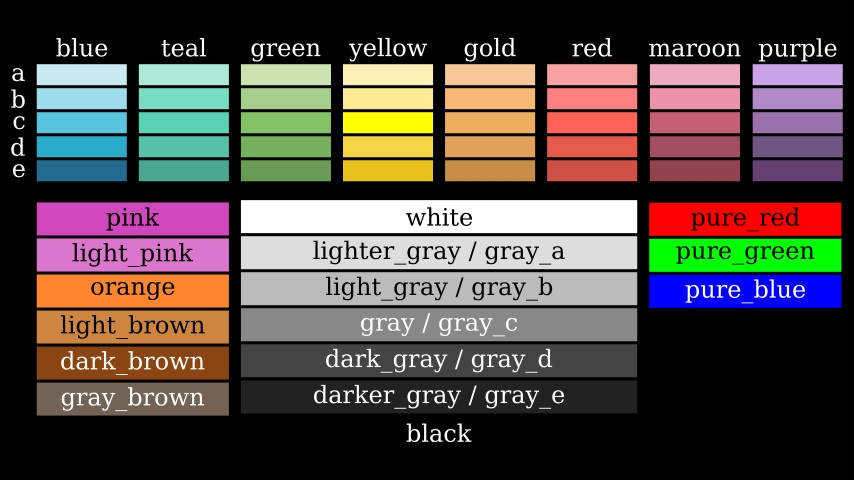
\includegraphics[width=0.8\textwidth]{part/图形化/manim/pic/基本图形/manim颜色.png}
    \caption{manim预置颜色}
    \label{fig:manim预置颜色}
\end{figure}


可以通过\codeinline{color}来设置图形的颜色。

\begin{lstlisting}[style=pythonstyle]
from manim import *

class ColorLineDemo(Scene):
    def construct(self):
        # 定义所有颜色系列及其不同深度
        color_groups = [
            [BLUE_E, BLUE_D, BLUE_C, BLUE_B, BLUE_A],        # blue 系列
            [TEAL_E, TEAL_D, TEAL_C, TEAL_B, TEAL_A],        # teal 系列
            [GREEN_E, GREEN_D, GREEN_C, GREEN_B, GREEN_A],   # green 系列
            [YELLOW_E, YELLOW_D, YELLOW_C, YELLOW_B, YELLOW_A], # yellow 系列
            [GOLD_E, GOLD_D, GOLD_C, GOLD_B, GOLD_A],        # gold 系列
            [RED_E, RED_D, RED_C, RED_B, RED_A],             # red 系列
            [MAROON_E, MAROON_D, MAROON_C, MAROON_B, MAROON_A], # maroon 系列
            [PURPLE_E, PURPLE_D, PURPLE_C, PURPLE_B, PURPLE_A], # purple 系列
            [PINK, LIGHT_PINK, ORANGE, LIGHT_BROWN, DARK_BROWN], # 单色系列
            [GRAY_BROWN, WHITE, LIGHTER_GRAY, LIGHT_GRAY, GRAY], # 灰色系列
            [DARK_GRAY, DARKER_GRAY, BLACK],                  # 深灰系列
            [PURE_RED, PURE_GREEN, PURE_BLUE]                # 纯色系列
        ]

        # 起始位置的 y 坐标
        y_start = 3
        # 每个颜色组的初始 x 坐标
        x_start = -6

        # 绘制每个颜色组及其深度
        for i, color_group in enumerate(color_groups):
            # 调整 x 坐标以便水平排列
            x_pos = x_start + (i * 1.6)
            for j, color in enumerate(color_group):
                # 创建每条线的y坐标偏移
                y_pos = y_start - (j * 0.6)
                line = Line(
                    [x_pos, y_pos, 0],
                    [x_pos + 1.2, y_pos, 0],
                    stroke_width=10,
                    color=color
                )
                # 动画显示线条
                self.play(Create(line), run_time=0.2)

        # 保持显示2秒
        self.wait(2)
\end{lstlisting}

\subsubsection{填充和透明度}
\label{subsubsec:Manim基本图形-填充和透明度}
可以通过\codeinline{fill\_color}和\codeinline{fill\_opacity}来设置图形的填充颜色和填充透明度。
\begin{lstlisting}[style=demostyle,numbers=none]
# 1.fill_color:
    类型: 字符串（颜色名称或十六进制颜色代码）
    描述: 指定图形的填充颜色。
    提示: 如果 fill_color 不是有效的颜色名称或十六进制颜色代码，则使用默认值 WHITE。

# 2.fill_opacity:
    类型: 浮点数或整数
    描述: 设置图形的填充透明度，取值范围为 0 到 1。
    默认值: 0
    提示: 如果 fill_opacity 小于 0 或大于 1，则使用默认值 0。
\end{lstlisting}

\begin{lstlisting}[style=pythonstyle]
# manim -pql 03Line_demo.py LineSample
from manim import *
class LineSample(Scene):
    def construct(self):
        self._lines()

    def _lines(self):
        # 1.创建简单的直线
        l1 = Line(
            [-1, 1, 0],
            [1, 1,0],
            fill_color=BLUE,
            fill_opacity=0.5,
            stroke_width=1,
        )
        self.play(Create(l1), run_time=0.5)

        l2 = Line(
            [-1, 0, 0],
            [1, 0, 0],
            fill_color=RED,
            fill_opacity=0.75,
            stroke_width=2,
        )
        self.play(Create(l2), run_time=0.5)

        c1 = Circle(
            radius=1,
            fill_color=BLUE,
            fill_opacity=0.5,
            stroke_width=1,
        )
        self.play(Create(c1), run_time=0.5)
\end{lstlisting}        


\section{坐标系}
\label{sec:Manim基本图形-坐标系}
没有引入坐标系之前，在绘制图形时，也有一个隐含的坐标系，它和屏幕的像素相关。

比如，我们之前示例中的各个图形，屏幕的中心就是坐标原点（$[0, 0]$）, 
横轴坐标的范围大概是 $[-3.5, 3.5]$，纵轴的坐标范围大概是 $[-4, 4]$，
这个范围与设置的视频分辨率有关，分辨率设置的越高的话，坐标范围越大。

\subsection{一维坐标系}
\label{subsec:Manim基本图形-一维坐标系}
数轴（\codeinline{NumberLine}）是最基本的一维坐标系，它的关键参数是
\begin{enumerate}[label=\arabic*)]
    \item \codeinline{x\_range}:设置数轴的范围和间隔
    \item \codeinline{length}:设置数轴的长度
\end{enumerate}
\begin{lstlisting}[style=pythonstyle]
# manim -pql 01NumberLineExample.py NumberLineExample
from manim import *

class NumberLineExample(Scene):
    def construct(self):
        # 第一条数轴：范围从 -10 到 10，步长为 2，长度为 10，包含数 字
        number_line_1 = NumberLine(
            x_range=[-10, 10, 2],  # 设置数轴范围为 -10 到 10，步长 为 2
            length=10,  # 设置数轴长度为 10
            include_numbers=True  # 在数轴上显示数字
        )
        number_line_1.to_edge(UP)  # 将第一条数轴移到屏幕上方

        # 第二条数轴：范围从 -3 到 3，步长为 0.5，长度为 12，包含数 字
        number_line_2 = NumberLine(
            x_range=[-3, 3, 0.5],  # 设置数轴范围为 -3 到 3，步长为 0.5
            length=12,  # 设置数轴长度为 12
            include_numbers=True  # 在数轴上显示数字
        )
        number_line_2.next_to(number_line_1, DOWN, buff=1)  # 将第二条数轴放在第一条数轴下方

        # 第三条数轴：范围从 -5 到 5，步长为 1，长度为 6，包含数字和箭头，旋转10度
        number_line_3 = NumberLine(
            x_range=[-5, 5 + 1, 1],  # 设置数轴范围为 -5 到 6，步长 为 1
            length=6,  # 设置数轴长度为 6
            include_numbers=True,  # 在数轴上显示数字
            include_tip=True,  # 在数轴的两端加上箭头
            rotation=10 * DEGREES  # 数轴旋转10度
        )
        number_line_3.next_to(number_line_2, DOWN, buff=1)  # 将第三条数轴放在第二条数轴下方

        # 动画显示三条数轴
        self.play(Create(number_line_1))
        self.play(Create(number_line_2))
        self.play(Create(number_line_3))

        # 保持场景显示2秒
        self.wait(2)

if __name__ == "__main__":
    from manim import config
    config.background_color = "#ffffff"  # 设置背景为白色
    scene = NumberLineExample()
    scene.render()
\end{lstlisting}           

\subsection{二维坐标系}
\label{subsec:Manim基本图形-二维坐标系}
\subsubsection{NumberPlane 实数平面}
\label{subsubsec:Manim基本图形-实数平面}
实数平面（\codeinline{NumberPlane}）是最基本的二绶坐标系，它的关键参数是
\begin{enumerate}[label=\arabic*)]
    \item \codeinline{x\_range}:设置\textcolor{YBXPurple}{X轴}横轴的范围和间隔
    \item \codeinline{y\_range}:设置\textcolor{YBXPurple}{Y轴}纵轴的范围和间隔
    \item \codeinline{x\_length}:设置\textcolor{YBXPurple}{X轴}横轴的长度
    \item \codeinline{y\_length}:设置\textcolor{YBXPurple}{Y轴}纵轴的长度
\end{enumerate}

\begin{lstlisting}[style=pythonstyle]
# manim -pql 01NumberPlaneExample.py NumberPlaneExample
from manim import *

class NumberPlaneExample(Scene):
    def construct(self):
        # 第一张网格：x 轴范围为 -4 到 11，y 轴范围为 -3 到 3，x 轴 长度为 3，y 轴长度为 2
        number_plane_1 = NumberPlane(
            x_range=(-4, 11, 1),  # 设置 x 轴范围为 -4 到 11，步长为 1
            y_range=(-3, 3, 1),   # 设置 y 轴范围为 -3 到 3，步长为 1
            x_length=3,  # 设置 x 轴的物理长度为 3
            y_length=2   # 设置 y 轴的物理长度为 2
        )
        number_plane_1.shift(LEFT * 2)  # 将第一张网格移到屏幕左侧

        # 第二张网格：x 轴范围为 -4 到 11，x 轴长度为 3，y 轴长度为 4（没有指定 y 轴范围）
        number_plane_2 = NumberPlane(
            x_range=(-4, 11, 1),  # 设置 x 轴范围为 -4 到 11，步长为 1
            x_length=3,  # 设置 x 轴的物理长度为 3
            y_length=4   # 设置 y 轴的物理长度为 4
        )
        number_plane_2.shift(RIGHT * 2)  # 将第二张网格移到屏幕右侧

        # 动画显示两张网格
        self.play(Create(number_plane_1))
        self.play(Create(number_plane_2))

        # 保持场景显示2秒
        self.wait(2)

if __name__ == "__main__":
    from manim import config
    config.background_color = "#ffffff"  # 设置背景为白色
    scene = NumberPlaneExample()
    scene.render()
\end{lstlisting}      

\subsubsection{ComplexPlane 复数平面}
\label{subsubsec:Manim基本图形-复数平面}

\begin{lstlisting}[style=pythonstyle]
# manim -pql 01ComplexPlaneExample.py ComplexPlaneExample
from manim import *

class ComplexPlaneExample(Scene):
    def construct(self):
        # 创建复平面，并添加坐标系
        plane = ComplexPlane().add_coordinates()

        # 创建第一个点，表示复数 2 + i，颜色为黄色
        d1 = Dot(plane.n2p(2 + 1j), color=YELLOW)  # 使用 n2p 将复数转换为平面上的点
        label1 = Tex("2+i").next_to(d1, UR, buff=0.1)  # 在点的右上 角添加标签 "2+i"

        # 创建第二个点，表示复数 -3 - 2i，颜色为黄色
        d2 = Dot(plane.n2p(-3 - 2j), color=YELLOW)  # 使用 n2p 将复 数转换为平面上的点
        label2 = Tex("-3-2i").next_to(d2, UR, buff=0.1)  # 在点的右 上角添加标签 "-3-2i"

        # 动画显示复平面、点和标签
        self.play(Create(plane))
        self.play(FadeIn(d1, label1))
        self.play(FadeIn(d2, label2))

        # 保持场景显示2秒
        self.wait(2)

if __name__ == "__main__":
    from manim import config
    config.background_color = "#fafafa"  # 设置浅色背景
    scene = ComplexPlaneExample()
    scene.render()
\end{lstlisting}        

\subsubsection{PolarPlane 极坐标平面}
\label{subsubsec:Manim基本图形-极坐标平面}
\codeinline{PolarPlane}是一个极坐标平面，它通过角度和与原点的距离来定位位置，经常被用于导航类的系统中， 与直角坐标相比，在这类系统中能极大的简化计算。 它的关键参数有：
\begin{enumerate}[label=\arabic*)]
    \item \codeinline{azimuth\_step}:分割的角度个数
    \item \codeinline{size}:极坐标在屏幕中显示的大小
    \item \codeinline{radius\_step}：极坐标半径的间隔
    \item \codeinline{radius\_max}：极坐标最大半径
\end{enumerate}


\begin{lstlisting}[style=pythonstyle]
# manim -pql 01PolarPlaneExample.py PolarPlaneExample
from manim import *

class PolarPlaneExample(Scene):
    def construct(self):
        # 创建极坐标平面
        plane = PolarPlane(
            azimuth_step=30,   # 设置方位角步长为 30 度
            size=6,            # 设置极坐标平面的大小为 6
            radius_step=1,      # 设置半径的步长为 1
            radius_max=3        # 设置最大半径为 3
        ).add_coordinates()     # 添加坐标轴的数字

        # 将极坐标平面居中放置
        plane.move_to(ORIGIN)

        # 动画显示极坐标平面
        self.play(Create(plane))

        # 保持场景显示2秒
        self.wait(2)

if __name__ == "__main__":
    from manim import config
    config.background_color = "#fafafa"  # 设置浅色背景
    scene = PolarPlaneExample()
    scene.render()
\end{lstlisting}      

\subsubsection{Axes 二维笛卡尔坐标轴}
\label{subsubsec:Manim基本图形-二维笛卡尔坐标轴}
二维的笛卡尔坐标系（\codeinline{Axes}）使用的比较多，它在平面坐标系之上，
又提供了更多的配置， 可以更加灵活的配置数轴，除了上面平面坐标系提到的那4个关键参数之外， 
还有2个配置坐标轴的参数也很重要：
\begin{enumerate}[label=\arabic*)]
    \item \codeinline{x\_axis\_config}:配置X轴如何显示的参数
    \item \codeinline{y\_axis\_config}:配置Y轴如何显示的参数
\end{enumerate}

\begin{lstlisting}[style=pythonstyle]
# manim -pql 01LogPlotExample.py LogPlotExample
from manim import *

class LogPlotExample(Scene):
    def construct(self):
        # 创建带有对数 y 轴的坐标系
        ax = Axes(
            x_range=[0, 10, 1],   # x 轴范围为 0 到 10，步长为 1
            y_range=[-2, 6, 1],   # y 轴范围为 -2 到 6，对数缩放
            x_length=6,           # x 轴长度为 6
            tips=False,           # 去掉轴的箭头
            axis_config={"include_numbers": True},  # 在轴上显示数字
            y_axis_config={"scaling": LogBase(custom_labels=True)},  # y 轴采用对数缩放
        )

        # 绘制 y = x^2 的函数曲线，注意 x_min 必须大于 0，因为 x=0  时，y 是负无穷
        graph = ax.plot(lambda x: x**2, x_range=[0.001, 10], use_smoothing=False)

        # 将坐标轴和函数曲线添加到场景中
        self.play(Create(ax), Create(graph))

        # 保持场景显示2秒
        self.wait(2)

if __name__ == "__main__":
    from manim import config
    config.background_color = "#ffffff"  # 设置浅色背景
    scene = LogPlotExample()
    scene.render()
\end{lstlisting}     



\subsection{三维坐标系}
\label{subsec:Manim基本图形-三维坐标系}
\subsubsection{ThreeDAxes 三维笛卡尔坐标系}
\label{subsubsec:Manim基本图形-三维笛卡尔坐标系}
三维的笛卡尔坐标系（\codeinline{ThreeDAxes}）与二维坐标系的参数类似，只是多了一个维度（Z轴）的配置， 其配置参数与X轴和Y轴类似。 
显示三维图形时，有2点需要额外注意，
\begin{enumerate}[label=\arabic*)]
    \item 场景要继承 \codeinline{ThreeDScene}
    \item 要调整下默认的相机位置，也就是视角的位置，默认视角是从Z轴顶部向下看的。
\end{enumerate}

\begin{lstlisting}[style=pythonstyle]
# manim -pql  01CoordinateSample.py  CoordinateSample
from manim import *

# 创建三维坐标轴并绘制一个蓝色圆形
class CoordinateSample(ThreeDScene):
    def construct(self):
        # 创建三维坐标轴，设置 y 轴的长度为 8
        axes = ThreeDAxes(y_length=8)

        # 创建一个蓝色的圆形，半径为 2
        circle = Circle(color=BLUE, radius=2)

        # 将坐标轴和圆形组合成一个 VGroup，以便同时显示
        vg = VGroup(axes, circle)

        # 默认的相机视角

        # 动画显示坐标轴和圆形
        self.play(Create(vg), run_time=2)

        # 暂停以查看最终场景
        self.wait()

# 运行场景
if __name__ == "__main__":
    from manim import config
    config.background_color = "#ffffff"  # 设置背景颜色为白色
    scene = CoordinateSample()
    scene.render()
\end{lstlisting}    

\begin{lstlisting}[style=pythonstyle]
# manim -pql  01CoordinateSample.py  CoordinateSample
from manim import *

# 创建三维坐标轴并绘制一个蓝色圆形
class CoordinateSample(ThreeDScene):
    def construct(self):
        # 创建三维坐标轴，设置 y 轴的长度为 8
        axes = ThreeDAxes(y_length=8)

        # 创建一个蓝色的圆形，半径为 2
        circle = Circle(color=BLUE, radius=2)

        # 将坐标轴和圆形组合成一个 VGroup，以便同时显示
        vg = VGroup(axes, circle)

        # 调整相机视角的代码 phi是与Z轴之间的角度，theta是围绕Z轴旋 转的角度
        self.set_camera_orientation(phi=75 * DEGREES, theta=30 * DEGREES)

        # 动画显示坐标轴和圆形
        self.play(Create(vg), run_time=2)

        # 暂停以查看最终场景
        self.wait()

# 运行场景
if __name__ == "__main__":
    from manim import config
    config.background_color = "#ffffff"  # 设置背景颜色为白色
    scene = CoordinateSample()
    scene.render()
\end{lstlisting}  


\begin{example}
    \exProblem
    实现全互联的神将网络
    \exSolution
    \begin{lstlisting}[style=pythonstyle]
    # manim -pql 02NeuralNetwoek_01.py
    from manim import *

    class NeuralNetwork(Scene):
        def construct(self):
            # 定义每一层的神经元数量
            #layer_sizes = [1, 8, 16, 8, 1]
            layer_sizes = [1, 8, 8, 1]
    
            # 定义每层神经元的位置
            layers = self.create_layers(layer_sizes)
    
            # 连接所有层的节点
            self.connect_layers(layers)
    
            # 保持显示
            self.wait(2)
    
        def create_layers(self, layer_sizes):
            """
            创建每一层的神经元，并返回各层的节点集合
            """
            layers = []
            x_position = -5  # 起始x坐标
            for layer_size in layer_sizes:
                layer = self.create_layer(layer_size, x_position)
                layers.append(layer)
                x_position += 2  # 各层间隔
    
            return layers
    
        def create_layer(self, layer_size, x_position):
            """
            创建单层神经元，并返回该层的节点集合
            """
            layer = VGroup()  # 创建一个组来包含这一层的所有节点
            y_start = -(layer_size - 1) / 2  # 起始y坐标
            for i in range(layer_size):
                neuron = Circle(radius=0.2, color=WHITE)  # 创建一个神经元（圆形）
                neuron.move_to([x_position, y_start + i, 0])  # 移动到指定位置
                layer.add(neuron)
                self.play(Create(neuron), run_time=0.1)  # 动画显示神经 元
    
            return layer
    
        def connect_layers(self, layers):
            """
            连接相邻层之间的所有神经元
            """
            for i in range(len(layers) - 1):
                layer1 = layers[i]
                layer2 = layers[i + 1]
                for neuron1 in layer1:
                    for neuron2 in layer2:
                        connection = Line(neuron1.get_center(), neuron2.get_center(), stroke_width=1, color=WHITE)
                        self.play(Create(connection), run_time=0.05)  # 动画显示连接线
    \end{lstlisting}
\end{example}


